% Vorbereitung: Vorbereitungsaufgaben bearbeiten
% Versuchsaufbau: Verwendete Apparatur, Beschreibung Funktionsweise/Nutzen mit Skizze/Foto
\section{Durchführung}
\label{sec:durchführung}
Die verwendete Schaltung zur Aufnahme der Franck-Hertz Kurve ist in \autoref{fig:app} gezeigt.
\begin{figure}[H]
	\centering
	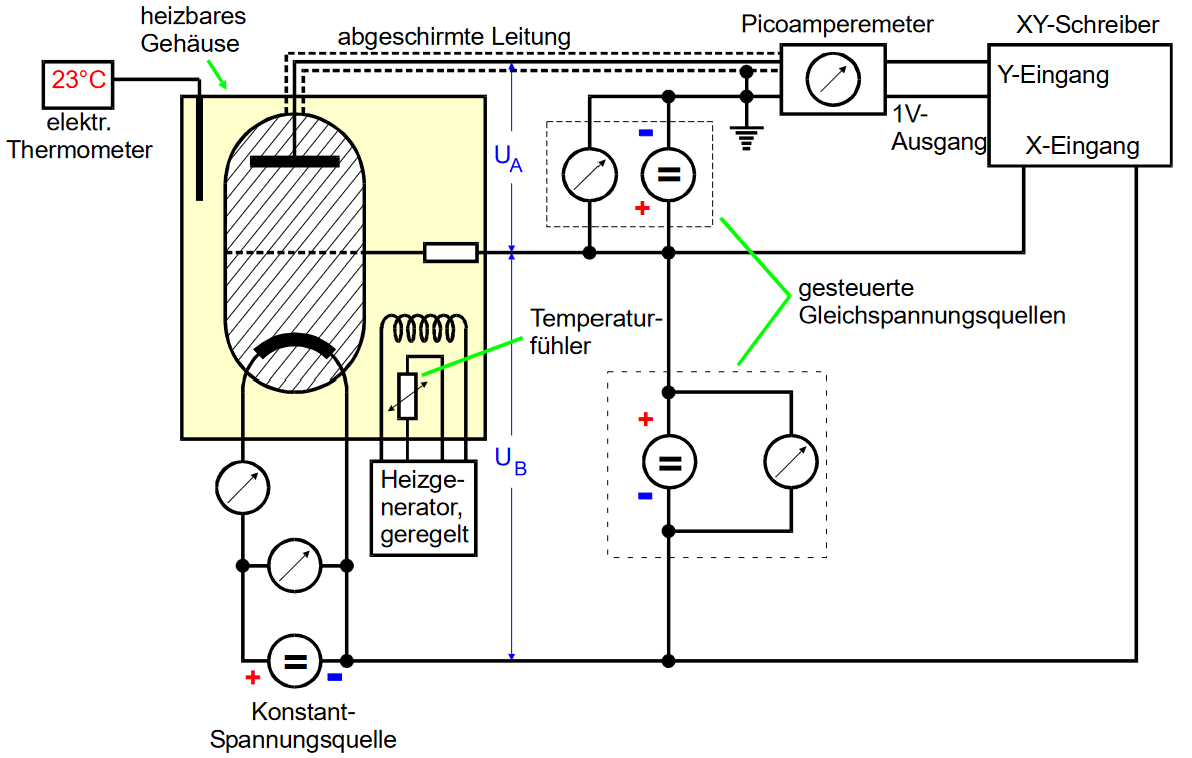
\includegraphics[width=0.75\linewidth]{content/grafik/apperatur.png}
	\caption{Die Schaltung zur Aufnahme der Franck-Hertz Kurve. \cite{franck}}
	\label{fig:app}
\end{figure}
Die Umgebungstemperatur $T$ wird mithilfe eines Heizgenerators gesteuert und schließlich an einem 
Thermometer abgelesen. Mit einen XY-Schreiber wird der Auffängerstrom in Abhängigkeit der zu betrachtenden Spannung aufgenommen.

Zu Beginn der Messung bei einer Raumtemperatur $T =\qty{24.3}{°C}$ wird der Auffängerstrom $I_A$ als Kurve in Abhängigkeit der Gegenspannung $U_A$ aufgenommen.
Die Beschleunigungsspannung ist dabei konstant bei $ U_B = \SI{11}{\volt}$ eingestellt. $U_A$ wird von $\SI{1}{\volt}$ bis $\SI{10}{\volt}$ hochgeregelt.
Der Vorgang wird für eine Temperatur $T =\qty{145}{°C}$ wiederholt. Daraufhin werden Kurven aufgenommen, bei denen eine Abhängigkeit der
Beschleunigungsspannung $U_B$ vorliegt. Diese wird von $\SI{0}{\volt}$ bis $\SI{55}{\volt}$ variiert. $U_A$ ist dabei zunächst auf $\SI{1}{\volt}$ und
anschließend auf $\SI{2}{\volt}$ eingestellt. Es werden je Messungen für eine Temperatur von $T = \qty{160}{°C}$ und $T = \qty{180}{°C}$ durchgeführt.
